\documentclass{article}
\usepackage[a4paper,margin=1in]{geometry}
\usepackage{amsmath,amssymb}
\usepackage{mdframed}
\usepackage{xcolor}
\usepackage{pgfplots}
\pgfplotsset{compat=1.18}


\setlength{\parskip}{1em}  % Set the space between paragraphs
\setlength{\parindent}{0pt}  % Remove the indentation at the beginning of paragraphs

\mdfsetup{
topline=false,
rightline=false,
bottomline=false,
linewidth=5pt,
innerleftmargin=15pt,
innerrightmargin=0pt,
skipabove=\baselineskip,
skipabove=1.2\baselineskip,
}

\definecolor{lightblue}{RGB}{160, 216, 239}
\definecolor{darkblue}{RGB}{40, 100, 158}

\begin{document}

\title{fonctions trigonometriques suite}
\author{B. Ruben}
\date{\today}

\maketitle

\section{les fonctions trigonometriques}

\begin{figure}[h!]
  \centering  
  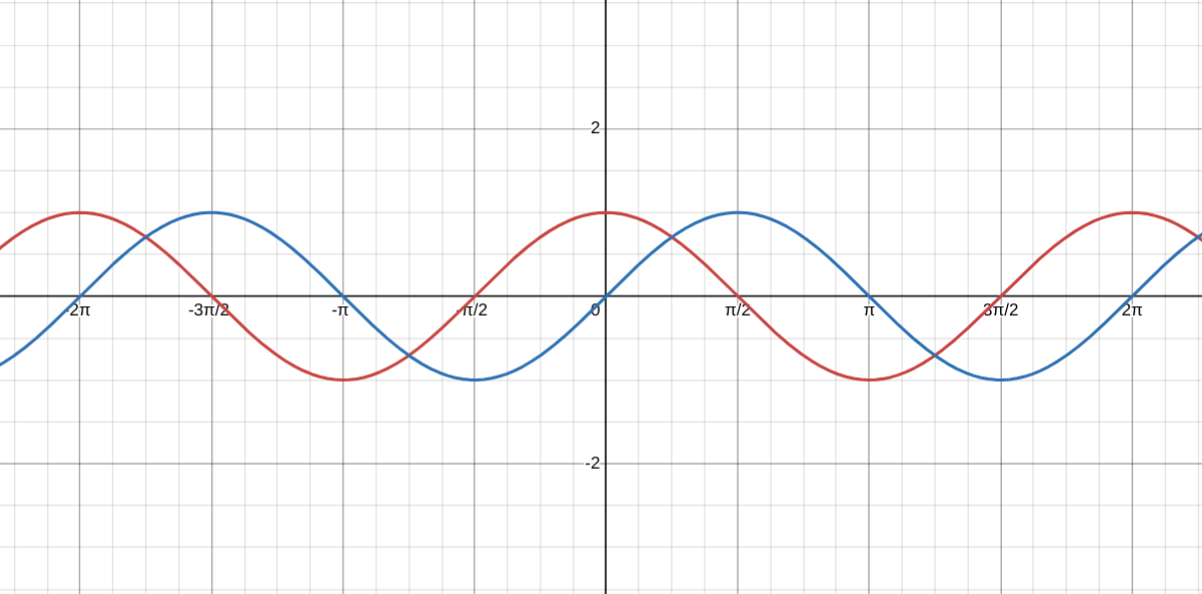
\includegraphics[width=1\textwidth]{./ftrig-image.png}
  \caption{fonctions trigonometriques}
  \label{fig:example}
\end{figure}



\end{document}
